\documentclass[a4paper,twoside]{article}

  \usepackage{verbatim}
   \usepackage{flushend}
\usepackage{epsfig}
\usepackage{subfigure}
\usepackage{calc}
\usepackage{amssymb}
\usepackage{amstext}
\usepackage{amsmath}
\usepackage{amsthm}
\usepackage{multicol}
\usepackage{pslatex}
\usepackage{apalike}
\usepackage{SciTePress}
\usepackage[small]{caption}

\subfigtopskip=0pt
\subfigcapskip=0pt
\subfigbottomskip=0pt

\begin{document}

\title{Model of Software and Hardware Infrastructure for Electrophysiology} 

\author{\authorname{Petr Je\v{z}ek\sup{1}, Roman Mou\v{c}ek\sup{2}, Jan \v{S}t\v{e}bet\'{a}k\sup{2}, Petr Br\r{u}ha\sup{2}}
\affiliation{\sup{1}New Technologies for the Information Society, \sup{2}Department of Computer Science and Engineering}
\affiliation{University of West Bohemia,}
\affiliation{Univerzitni 8, 306 14,}
\affiliation{Pilsen, Czech Republic}
\email{jezekp@ntis.zcu.cz, \{moucek, stebjan, pbruha\}@kiv.zcu.cz}
}

\keywords{neuroinformatics, electroencephalography, event-related potentials, infrastructure, data management, semantic web, analytic tool, Semantic Framework}

\abstract{Large amounts of EEG/ERP (electroencephalography, event-related potential) data, various data formats and non-standardized domain description lead to incompatible results and interpretations of EEG/ ERP experimental data/metadata and to difficult communication between interested laboratories. Authors' research group has solved these problems and has contributed to the building of a neuroinformatics infrastructure by developing and integrating data management and analytic tools for EEG/ERP research. The model of the software and hardware infrastructure for electrophysiology, and the context and architecture of the developed EEG/ERP Portal, serving to manage, share and process EEG/ERP experiments, are presented. Other additional tools are briefly described.}

\onecolumn \maketitle \normalsize \vfill
\section{\uppercase{Introduction}}

\noindent Our research group specializes in the research of brain activity; especially attention of drivers  and seriously injured people is investigated. We widely use the methods of  electroencephalography (EEG) and event related potentials (ERP). EEG/ERP experiments usually take long time and produce~a lot of data. Since we repeatedly need to collect, store and analyze experimental data and metadata, we have faced several difficulties, for example, the long-term storage of data and metadata, re-analysis of raw data, sharing of data/metadata, and design of various experimental protocols. To solve these difficulties the complex software and hardware infrastructure for electrophysiology have been gradually designed and partly implemented.

As the members of the Czech National Node of International Neuroinformatics Coordinating Facility (INCF) \cite{incf} we participate in definition and development of standardized formats for electrophysiology research. Our efforts, following INCF recommendations \cite{incf-sustainability-report}, resulted in the central custom solution - the EEG/ERP Portal.

In this paper we briefly present the infrastructure solutions in neuroscience as they are provided by the member countries of INCF. Then the basic ideas and the model of software and hardware infrastructure for electrophysiology is introduced.  In the next sections the overall concept and architecture of the EEG/ERP Portal is described. Since we need to register the Portal as a recognizable data source, we also implemented the Semantic Framework module (Section \ref{sec:Semantic Web Extension}) that enables users transformation of the common object oriented source code into semantic web languages \cite{key-the-semantic-web}. Semantic gaps between the object-oriented code and its semantic web representation are bridged by extension of the object-oriented code using Java annotations. The EEG/ERP Portal is also supposed to be integrated with various external tools; these are described in Section VI.

\section{\label{State of the Art}\uppercase{State of the Art}}

\noindent The neuroinformatics infrastructure is being built in several INCF national nodes in parallel. The INCF portal~\cite{incf} includes, for example, a software center for easy storage and sharing of neuroinformatics software tools, a content management system for national nodes presentation and provides access to supercomputing resources for the neuroinformatics community.

The Neuroscience Information Framework (NIF)~\cite{NIF-Neuroinformatics} is a dynamic inventory of registered Web-based neuroscience resources containing data, materials, and tools. It advances research in neuroscience by enabling access to public research data and tools through an open source environment. Currently more than 4,000 sources are registered within NIF.

The Carmen portal~\cite{carmen} provides storage of experimental data, metadata and analysis code. Users can also analyze their experimental data. Their analytical tools are implemented as web services. Within the Japan National Node, neuroinformatics databases are organized and shared with the public in platforms. The platforms serve as storages of experimental data and documents; some of them provide analytic tools.

Semantic web solutions for EEG/ERP data management focus mainly on building ontologies. The ontology built within the NEMO project provides formal semantic definitions of concepts in ERP domain, including ERP patterns, spatial, temporal, functional (cognitive/behavioral) attributes of these patterns, and data acquisition and analytic methods and parameters \cite{neuralontologies}.

The fundamental method for obtaining ERP components from the EEG signal is averaging. The methods used for ERP components detection include the matching pursuit algorithm, wavelet transform and Hilbert-Huang transform~\cite{ciniburk}.

\section{\label{Model}\uppercase{Model of software and hardware infrastructure}}

\noindent The basic idea of the model of the software and hardware infrastructure for electrophysiology comes from the set of main activities performed by researchers during electrophysiological experiments. First of all, researchers present a~hypothesis and design a~protocol for a~specific experiment. Then they perform the experiment and collect data and related metadata. During the experiment they have to synchronize the EEG signal obtained from the scalp of the tested subject with presented stimuli. Second, they analyse the data using various processing methods, interpret the data and publish results. In the long term, they do not care about the data and lose them. The biggest problems for science are the following ones: since data are not published, conclusions and interpretations cannot be later reproduced or verified, the methods used for data analysis are lost or their detailed parameters are not later traceable.

The basic aim of building the software and hardware infrastructure for electrophysiology is to increase both effectiveness and efficiency of scientific research in this field. The integrated system is considered as a service (compare to~\cite{fgibson:Watson2007}) providing usually the web-based interface. The main features of this service include a long-term and sustainable storage of data and related metadata collected from experiments, various methods for data processing, workflows for data processing and sharing of data, documents, methods and workflows in groups.

The software infrastructure with the central EEG/ERP portal is shown in Fig.~\ref{fig:Component Model of EEG/ERP Infrastructure}. The hardware infrastructure includes stimulators for ERP experiments and complex electronic switches for synchronization of impulses.

Sharing is very helpful for scientific community.  However, the present organization of science does not support it entirely. Scientists usually want to be the first to publish their ideas or results to gain recognition and money for their future research. Therefore it is not possible to fully open publication of ideas, data, or processing methods at every stage of the scientific process. As the result, sharing of knowledge has to be limited at least at early stage of the scientific process to defined groups of people. These groups can be gradually enlarged as the scientific process continues. Finally, after successful publication, the full access to data and to used methods is possible. It is clear that some data, for example, personal data of tested subjects have to be secured according to law. Laws or other privacy issues can even prevent any sharing of some data. After reading the paper other researchers can be interested in the data or their processing. For example, they want to use the same methods or workflows, which are applied to their data or they want to use original data to verify their own methods. Then new valuable results available for publication can be produced with adequate effort.

\section{\label{EEG/ERP Portal}\uppercase{EEG/ERP Portal - Context}}

\noindent The purpose of the EEG/ERP Portal is to serve as a~managing tool for EEG/ERP experiments. It enables interested laboratories sharing and interchange of the stored experiments (data, metadata,  experimental scenarios, etc.). The features of the EEG/ERP Portal also include sharing of knowledge, working in groups, content management system, and full-text search.

The EEG/ERP Portal is developed as an open source accepting INCF recommendations \cite{incf-sustainability-report}. The Portal does not require any special software installation, only a~web browser is needed.

The data are protected by the system of user accounts with defined user roles. Individual users are grouped into self-managed groups. On the basis of activities that the user can perform four user roles are recognized (Reader, Experimenter, Group Administrator, and Supervisor). The user who wants to upload or download experiments has to to create an account and to become a~member of at least one group. The user can create an account within the EEG/ERP Portal directly or he/she can use his/her Facebook account (this account is synchronized with the Portal account after the first login).

We prepared a simple wizard that guides the logged user through the process of adding an experiment. Each experiment contains raw data supplemented by related metadata. We defined a set of metadata which the user is instructed to fill in through the prepared forms. These metadata are organized in several semantic groups (experimental scenario, experimenters and tested subjects, used hardware, description of raw data, etc.). The experimenter can also decide if the experiment is private or public. Public experiments are downloadable for all registered users (without personal data of tested subjects), while private experiments are downloadable only within the experimenter's group.

\begin{figure*}
	\centering
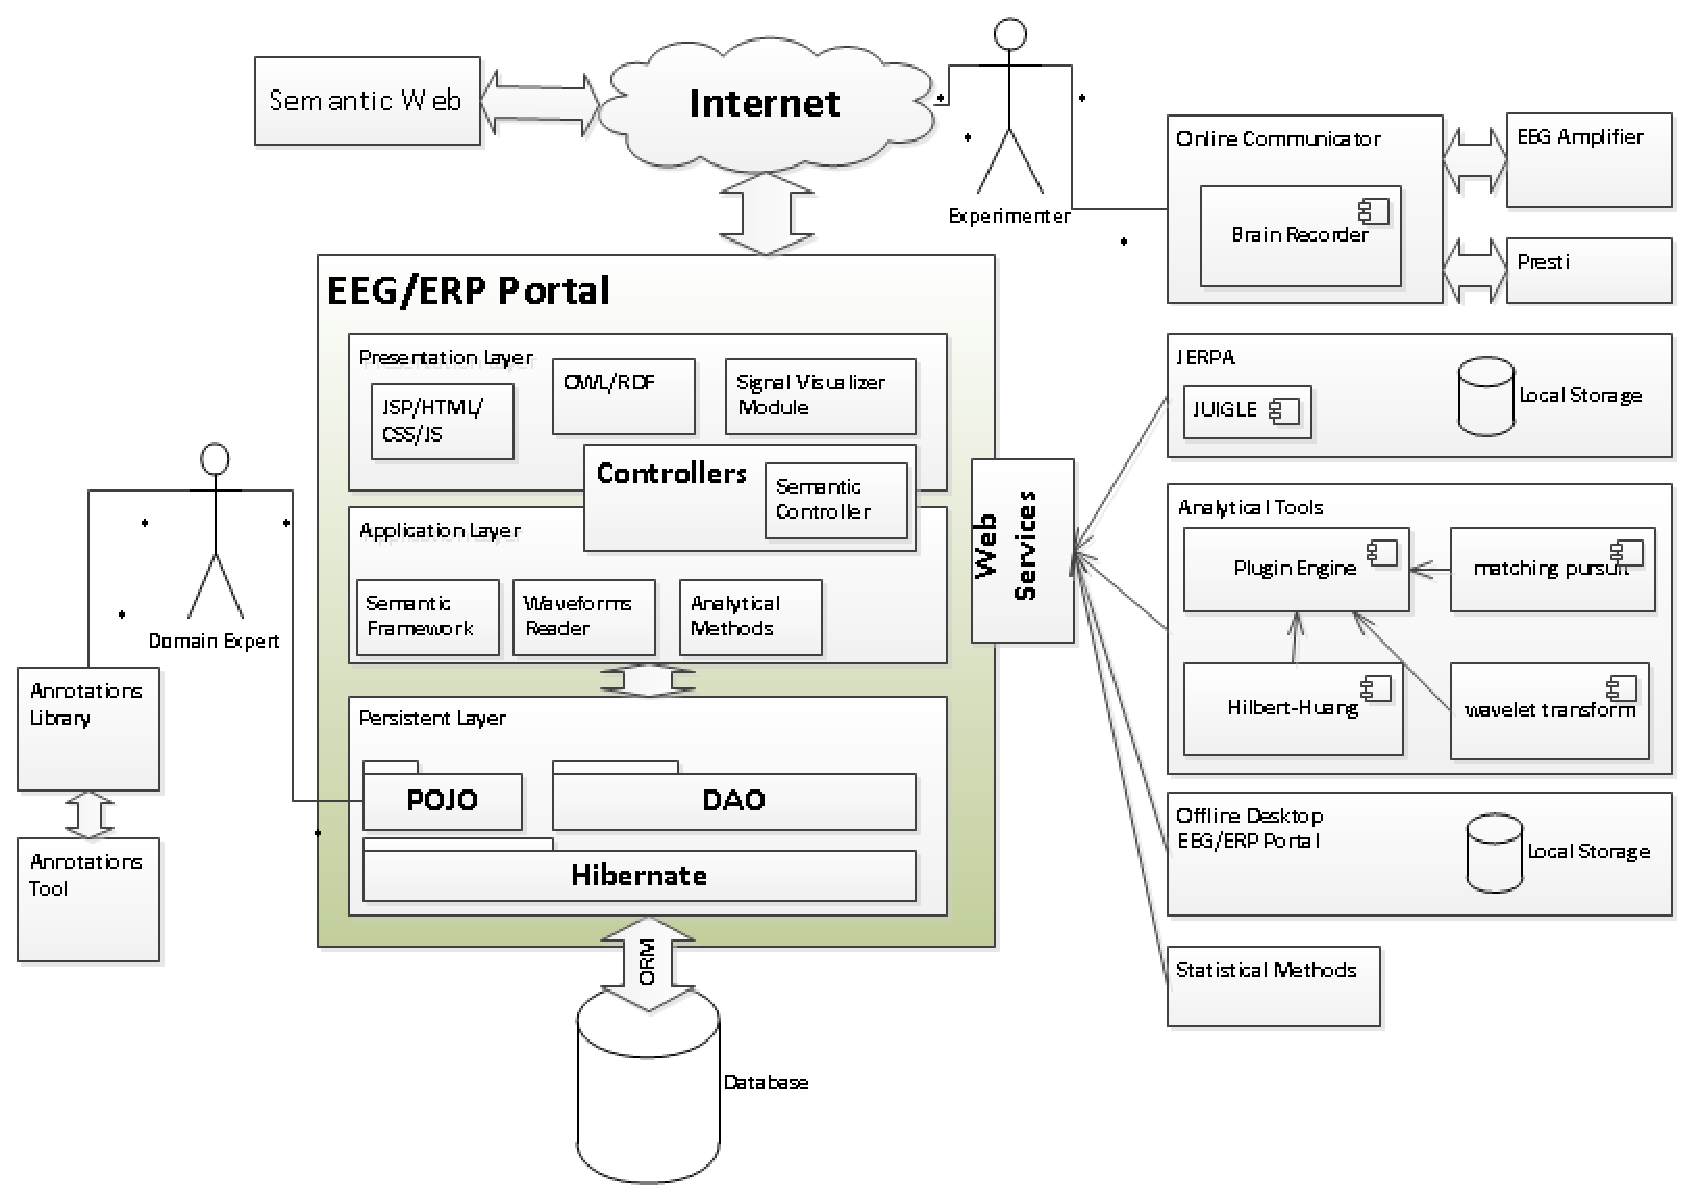
\includegraphics[width=15cm, height=10cm]{component_model_2}

\caption{\label{fig:Component Model of EEG/ERP Infrastructure}Component Model of EEG/ERP Infrastructure}

\end{figure*}

\begin{comment}
\section{Architecture}
%
During the development of the EEG/ERP portal the layered architecture, which ensures a high level of abstraction that facilitates adding a further functionality, is strictly required. Since our project uses open source technologies, many third-party libraries, stored in public repositories, are used. We successfully use Maven~\cite{maven} for building the project and managing custom and imported libraries.

\subsection{Persistent Layer}
The persistent layer uses Hibernate framework~\cite{hibernate} for object-relational mapping and Data Access Objects (DAO). The database server is Oracle 11g. The data model includes tables for storing EEG/ERP data and metadata, experimental scenarios, possible metadata extensions (without a necessity to change the basic ERA model), articles, tested subjects, information about users and research groups. Most attributes are obligatory. Due to the large number of database records a powerful search engine is requested. Therefore we use Hibernate Search based on the Apache Lucene full text search engine.

\subsection{Application Layer}
Application and presentation layers are designed and implemented using the Spring technology~\cite{spring} (including Spring MVC and Spring Security). When significant occasions occur (e.g. user registration or request for assignation to any group), the user is notified by e-mail through a~simple mailing center. Recently we have added modules facilitating data search, publishing, data download, data sharing, and management of users and their accounts.

\subsection{Presentation Layer}
The presentation layer is implemented using Java Server Pages with JSTL (Standard Tag Library). A~unified design of the pages is ensured using CSS (Cascading Style Sheets). Specific dynamic behavior of individual pages (table sorting, records filtering, etc.) is provided by JavaScript.
\end{comment}

\section{\label{sec:Semantic Web Extension}\uppercase{Semantic Web Extension}}

%\subsection{Difficulties with Semantic Web}
\noindent Before we started the registration of the EEG/ERP Portal as a recognizable neuroscience data source within the NIF \cite{NIF-Neuroinformatics}, we had described EEG/ERP experiments by a suitable ontology. The Semantic Web uses a~triple oriented representation described by Resource Description Framework (RDF) and its extension Ontology Web Language (OWL). Despite advantages that the Semantic Web (semantic description of stored data) brings, the EEG/ERP Portal is designed using object oriented modeling (OOM).

There are fundamental differences in richness of semantics between OOM and OWL.
\begin{comment}OWL is based on description logic and open world assumption. When some information is missing, we cannot decide if it is true or false. On the other hand, OOM deals with closed world assumption. When some information is missing, it is always considered to be false. \end{comment}
At least some of the semantic gaps are needed to be bridged.

\subsection{\label{subsec:Existing Approaches}Existing Approaches}
We tested several frameworks to enrich an object oriented code by missing semantics. ActiveRDF \cite{ActiveRDF} is a~library for accessing RDF data from Ruby programs. eClass \cite{Web-Information-Representation} is an extended Java class with changed syntax that contains additional information about fields and methods. The Semantic Object Framework \cite{SOF} adds missing semantics using embedded comments.

The tested frameworks are difficult to use either because they do not include suitable means for adding missing semantics, or they require a modification in common programming syntax.

\section{\uppercase{External Libraries and Tools}}

\noindent Since the EEG/ERP Portal cooperates with a set of associated submodules we implemented several communication interfaces for external tools. The tools working with the data stored in the EEG/ERP Portal can be divided into two groups. The first group includes tools that are accessible through an internet browser. These tools are implemented as stand-alone libraries integrated within the EEG/ERP Portal directly. The second group of tools includes desktop tools that are run locally on the user's computer. The desktop tools access data in the EEG/ERP Portal and manage them locally.

\subsection{Libraries of EEG/ERP Portal}

The libraries, implemented outside the system, are gradually added into the EEG/ERP Portal. The libraries are simultaneously placed into the open source repositories where they can be used by the interested community.

\subsubsection{Semantic Framework}

With regards to the difficulties mentioned in Section~\ref{subsec:Existing Approaches} we decided to implement a custom framework based on common programming technologies. It resulted in the development of the Semantic Framework that uses Java Annotations \cite{JavaAnnotations}. These annotations enable us to add advanced OWL constructs into the object oriented code. The Semantic Framework uses the modified JenaBean \cite{jena} in combination with the OWL API \cite{owl}. The JenaBean was extended by the set of annotations mapped to appropriate OWL constructs~\cite{DBLP:conf/iceis/MoucekJ10}.


\subsubsection{Waveforms Reader}

The data obtained during the EEG/ERP experiments are stored in the format given by the used analogue-digital converter. We provide a module for playing the stored signal in the web-based interface of the EEG/ERP Portal. The Waveforms Reader separates individual waveforms that are visualized using HTML5 and CSS3 technologies. The rendering is smooth even if the signal is sought or zoomed.

\subsubsection{Analytic Methods}

EEG/ERP data are supposed to be further processed. We implemented the methods described in Section \ref{State of the Art} as single libraries. When the user executes a~method, this method is running in a separate thread in the background. When the execution of the method ends, the results are visualized in a~chart. It ensures that a parallel work may be done although the execution of the methods may be time-consuming.

\subsection{External Tools}

 External tools work independently of the EEG/ERP Portal. The EEG/ERP Portal provides an interface for accessing stored experiments using Web Services technology. The Apache CXF service framework is used. The Web Service interface provides several methods for accessing users experiments with their data, metadata and scenarios. The Web Service is secured by user credentials. When any request for other functionality occurs the provided interface can be extended. An interested client only implements a Web Service client.

\subsubsection{JERPA}

JERPA \cite{DBLP:conf/biostec/JezekM11} is a solution for visualization of EEG/ERP records. We extended the present solution about the possibility to download experiments from the EEG/ERP Portal. The user can download data of his/her experiments to the local storage and visualize them. The functionality for uploading a new experiment to the EEG/ERP Portal is also provided. The local storage is synchronized with the EEG/ERP Portal in regular intervals, then the local storage is always up-to-date.

\subsubsection{Analytic Tools}

Since processing of analytic methods is a~time consuming task we designed and implemented the system running on the separate server. This system implements analytic methods described in Section \ref{State of the Art}. The system contains a simple web-based interface where the user can list available methods and accessible server resources. The implemented methods are accessed using the Web Service as well. When any user wants to use this system he/she has to register.

\subsubsection{Offline EEG/ERP Portal}

Since there are many situations in which the Internet connection is not available during performing experiments, we prepared an offline (simplified) version of the EEG/ERP Portal as a~desktop application. The performed experiments are stored in the local storage. If Internet connection is available, the local storage is synchronized with the EEG/ERP Portal.

\subsubsection{Statistical Methods}

The library of statistical methods was implemented as a standalone product that runs on the separate server as well. Currently we have implemented one way and two way analysis of variance (ANOVA) and one way and two way multivariate analysis of variance (MANOVA).

\subsubsection{Brain Recorder}

We use the Brain Vision Recorder for collecting data from EEG/ERP experiments. The digitalized signal is stored in the local computer. The experimenter uploads this signal to the EEG/ERP Portal using the web-based wizard.

\subsubsection{Annotation Tool}

Since we provide the EEG/ERP experiments in the Semantic Web form using the Semantic Framework, the domain expert has to prepare a~set of annotated POJO objects. The annotation tool is a~standalone system that allows users to load POJOs from the persistence layer of the EEG/ERP Portal and annotate them. These annotated POJOs are exported from the Annotation Tool and integrated within the EEG/ERP Portal.

%
\section{\uppercase{Conclusion}}
%
\noindent 
The presented software and hardware infrastructure combines research in informatics with research in electrophysiology. Its aim is to help researchers in their work, which includes especially long-term collection, maintenance, usage and share of EEG/ERP data and related tools. The set of metadata is defined reflecting experience from experiments carried out in our laboratory, medical expertise provided by the University Hospital in Pilsen, INCF recommendations, and analysis of related books and scientific papers. The central point of the infrastructure, the EEG/ERP Portal, is being developed as an open source using common, basically object oriented technologies.

Since the registration of the EEG/ERP Portal as a recognizable data source requires providing its ontological description, transformation of the object oriented code into the semantic web technologies is required. The Semantic Framework provides this transformation and adds missing semantics using Java Annotations. The integration of the developed framework into the EEG/ERP Portal ensures the online serialization of the stored experiments into semantic web languages. Since processing of EEG/ERP experiments includes a~usage of a~large set of methods, the ways to run these methods were briefly presented.

Our future work will focus on expansion and improvement of the infrastructure. It includes building of the limited social network within the EEG/ERP Portal, cooperation of the Portal with social networks used by the community, the full registration of the EEG/ERP Portal within NIF, extensive work on the methods for EEG/ERP signal processing and building of workflow patterns. An equally important task is to continue in the standardization of data and metadata structures.
%
\section*{Acknowledgements}
\noindent The work was supported by the UWB grant SGS-2010-038 Methods and Applications of Bio- and Medical Informatics.

%\vfill
\bibliographystyle{apalike}
{\small
\bibliography{bibliography}}


\vfill
\end{document}

